\documentclass[12 pt, letterpaper]{exam}
\usepackage{amsfonts}
\usepackage{graphicx}
\usepackage{amsthm}
\usepackage{amssymb}
\usepackage{amsmath}
\usepackage{enumerate, mathrsfs}
\usepackage[framed,indented,numbered,autolinebreaks,useliterate]{mcode}
\printanswers

\theoremstyle{definition}
\newtheorem{ex}{Example}
\newtheorem{df}{Definition}
\newtheorem{thm}{Theorem}
\newtheorem{prob}{Problem}

\newcommand{\suchthat}{\,\Big{|}\,}
\newcommand{\ZZ}{\mathbb{Z}}
\newcommand{\QQ}{\mathbb{Q}}
\newcommand{\NN}{\mathbb{N}}
\newcommand{\RR}{\mathbb{R}}
\newcommand{\CC}{\mathbb{C}}
\newcommand{\dd}{\,\,\textrm{d}}
\printanswers

% \firstpageheader{Math 3900 Spring 2019}{Homework 5}{Instructor:  J. Haga}
 
% READ THIS:

% If you're going to adjust this code to formulate your own homework, then please comment (with a %) the above line and uncomment the line below (and change the last names of the mathematicians to your group members' last names in alphabetical order).

\firstpageheader{Math 3900 Spring 2018}{Homework 5}{Arnaudo, Mellen, Rawson}

\begin{document}
\begin{questions}
\question[50] Use the data below to construct a Hermite interpolant of the function $$f(x) = x^2+3x\sin(2x)-1:$$
\begin{align*}
\begin{array}{l|rrl}
x	&	f(x)		&	f'(x)		\\
\hline
1.3	&	 2.700455350	&	 -2.537228161	\\
1.8	&	-0.149610394	&	 -7.412552226	\\
2.4	&	-2.412385184	&	  3.071491535	\\
2.9	&	 3.367961039	&	19.81423306	
\end{array}
\end{align*}
Use your polynomial to approximate $f(2)$.  Use Theorem 3.9 to upper-bound the absolute error in this approximation.
\begin{solution}
    We started by constructing the lagrange interpolating polynomials:
    \begin{align*}
        \begin{array}{l|rrl}
            i	&	L_{3, i}(x)		&	L'_{3, i}(x)		\\
            \hline
            0	&	\frac{(x-1.8)(x-2.4)(x-2.9)}{-0.88}	&    -3.40909x^2 + 16.1364x - 18.75	    \\
            1	&	\frac{(x-1.3)(x-2.4)(x-2.9)}{0.33}	&	 9.09091x^2 - 40x + 41.9697	\\
            2	&   \frac{(x-1.3)(x-1.8)(x-2.9)}{-0.33}	&	 -9.09091x^2 + 36.3636x - 34.3333	\\
            3	&	\frac{(x-1.3)(x-1.8)(x-2.4)}{0.88}	&	 3.40909x^2 - 12.5x + 11.1136
        \end{array}
    \end{align*}

    Using the equations for $H_{n,j}$ and $\hat{H}_{n,j}$, we can got all of the equations:
    \begin{align*}
        \begin{array}{l|rrl}
            i	&	H_{3, i}(x)		&	\hat{H}_{3, i}(x)		\\
            \hline
            0	&	(1-2(x-1.3)(-3.5340))\frac{(x-1.8)^2(x-2.4)^2(x-2.9)^2}{0.7744}   & (x-1.3)\frac{(x-1.8)^2(x-2.4)^2(x-2.9)^2}{0.7744}  \\
            1	&	(1-2(x-1.8)(-0.5758))\frac{(x-1.3)^2(x-2.4)^2(x-2.9)^2}{0.1089}	& (x-1.8)\frac{(x-1.3)^2(x-2.4)^2(x-2.9)^2}{0.1089}  \\
            2	&   (1-2(x-2.4)(0.5757))\frac{(x-1.3)^2(x-1.8)^2(x-2.9)^2}{0.1089}	& (x-2.4)\frac{(x-1.3)^2(x-1.8)^2(x-2.9)^2}{0.1089} \\
            3	&	(1-2(x-2.9)(3.5340))\frac{(x-1.3)^2(x-1.8)^2(x-2.4)^2}{0.7744}	& (x-2.9)\frac{(x-1.3)^2(x-1.8)^2(x-2.4)^2}{0.7744}	
        \end{array}
    \end{align*}

    \newpage
    Which gives us the Hermite interpolant of:
    $$H(x) = 2.700455350*(1-2(x-1.3)(-3.5340))\frac{(x-1.8)^2(x-2.4)^2(x-2.9)^2}{0.7744}$$
    $$-0.149610394*(1-2(x-1.8)(-0.5758))\frac{(x-1.3)^2(x-2.4)^2(x-2.9)^2}{0.1089}$$
    $$-2.412385184*(1-2(x-2.4)(0.5757))\frac{(x-1.3)^2(x-1.8)^2(x-2.9)^2}{0.1089}$$
    $$+3.367961039*(1-2(x-2.9)(3.5340))\frac{(x-1.3)^2(x-1.8)^2(x-2.4)^2}{0.7744}$$
    $$-2.537228161*(x-1.3)\frac{(x-1.8)^2(x-2.4)^2(x-2.9)^2}{0.7744}$$
    $$-7.412552226*(x-1.8)\frac{(x-1.3)^2(x-2.4)^2(x-2.9)^2}{0.1089}$$
    $$+3.071491535*(x-2.4)\frac{(x-1.3)^2(x-1.8)^2(x-2.9)^2}{0.1089}$$
    $$+19.81423306*(x-2.9)\frac{(x-1.3)^2(x-1.8)^2(x-2.4)^2}{0.7744}$$

    Using $H(2)$, we approximate $f(2)$, which gives us $-1.5408$.

    We used this MATLAB code to calculate our values and our error:
    \begin{lstlisting}
syms x;

f(x) = x^2+3*x*sin(2*x)-1;
H(x) = 
2.700455350*(1-2*(x-1.3)*(-3.5340))*((x-1.8)^2*(x-2.4)^2*(x-2.9)^2)/(0.7744)
-0.149610394*(1-2*(x-1.8)*(-0.5758))*((x-1.3)^2*(x-2.4)^2*(x-2.9)^2)/(0.1089)
-2.412385184*(1-2*(x-2.4)*(0.5757))*((x-1.3)^2*(x-1.8)^2*(x-2.9)^2)/(0.1089)
+3.367961039*(1-2*(x-2.9)*(3.5340))*((x-1.3)^2*(x-1.8)^2*(x-2.4)^2)/(0.7744)
-2.537228161*(x-1.3)*((x-1.8)^2*(x-2.4)^2*(x-2.9)^2)/(0.7744)
-7.412552226*(x-1.8)*((x-1.3)^2*(x-2.4)^2*(x-2.9)^2)/(0.1089)
+3.071491535*(x-2.4)*((x-1.3)^2*(x-1.8)^2*(x-2.9)^2)/(0.1089)
+19.81423306*(x-2.9)*((x-1.3)^2*(x-1.8)^2*(x-2.4)^2)/(0.7744);

y = 2;
% print vals
disp('f(2)')
double(f(y))
disp('H(2)')
double(H(y))
disp('abs error')
vpa(double(abs(f(y) - H(y))))

% calulate error
n = 3;
xvals = [1.3 1.8 2.4 2.9];

numerator = 1;
for i = 1:3
    numerator = numerator * (y - xvals(i))^2;
end

% get the fractional part of the error
fraction = numerator / factorial(2 * n + 2);

% get 8th derivative of the function
derivs(x) = diff(f);
for i = 2:8
    derivs(x) = diff(derivs);
end
derivs(x)

% bounded derivative
g(x) = 768 * abs(x) + 3072;

bounded_error = fraction * g(2.9);
disp('error')
vpa(double(bounded_error))
    \end{lstlisting}

Given Theorem 3.9, our error will be $7.7778*10^{-8} \times f^{(8)}(\xi(x))$. We used the MATLAB code above to determine that the eighth derivative of $f$ is $768(x*sin(2x)-4cos(2x))$, which we can bound using the triangle inequality. This gives us that the eighth derivative is $\leq 768*|\xi(x)| + 3072$. Given this function, we can bound $\xi(x)$ by 2.9, as that will give us the largest possible value for this function. Using all of that, we find our bounded error to be 0.00041216. This bounded error agrees with our absolute error, which was 0.0000007186.

\end{solution}
\question[50] Determine the oscillating polynomial for $f(x) = \sin(x)$ by utilizing data at $0$, $\frac{\pi}{12}$, $\frac{5\pi}{12}$, $\frac{7\pi}{12}$, with $m_0=m_1=m_2=m_3=2$.
    \begin{solution}
        Here is the matlab code to solve this. Some of the code is too long to fit in the box so I continued it on the next line but I don't believe MatLab supports this so you might have to put it all on one line to run it:
        \begin{lstlisting}
close all
clear all
clc
    
syms a b c d e f g h i j k l x;

% Get the functions to find the values we want our polynomial to have
F(x) = sin(x);
FP(x) = diff(F(x));
FPP(x) = diff(FP(x));

% These are the x values we are given
xVals = [0, pi/12, 5*pi/12, 7*pi/12];

% Form the polynomial with variables for the coefficients
P(x) = a+b*(x)+c*(x^2)+d*(x^3)+
    e*(x^4)+f*(x^5)+g*(x^6)+h*(x^7)+
    i*(x^8)+j*(x^9)+k*(x^10)+l*(x^11);
PP(x) = diff(P(x));
PPP(x) = diff(PP(x));

% Set the polynomial equal to the constrains we set
E(x) = P(x) == F(x);
EP(x) = PP(x) == FP(x);
EPP(x) = PPP(x) == FPP(x);

% Create the matrix of linear equations
[A, B] = equationsToMatrix([E(xVals(1:4)), EP(xVals(1:4)), EPP(xVals(1:4))]);
    
% Solve the system of linear equations to get the coefficients
V = linsolve(A,B);

% Create the polynomial we were looking for S(x)
S(x) = V(1)+V(2)*(x)+V(3)*(x^2)+V(4)*(x^3)+
    V(5)*(x^4)+V(6)*(x^5)+V(7)*(x^6)+V(8)*(x^7)+
    V(9)*(x^8)+V(10)*(x^9)+V(11)*(x^10)+V(12)*(x^11);

% This plot shows our P(x) side by side with sin(x)
fplot([S(x), F(x)])

% Show the coefficients
vpa(double(V(1:12)))

$ These are the coefficients of the function:
V = 
     0
     1.0
     0
    -0.16666666630844645391462677253003
    -0.0000000054831881676034074194814167094343
     0.0083333669819250985599801140324416
    -0.00000010700146029082436262294350005908
    -0.00019821944419390222181728833383829
    -0.00000020848831200249861555651045928045
     0.0000028913351902119091380255564566193
    -0.000000050627456284926279935893037075292
    -0.000000016166820580423160280797751525185
        \end{lstlisting}
        \newpage
        The function did a good job of resembling sin(x) on the interval. On the graph below the blue line is our function and the orange line is sin(x):
        \begin{center}
            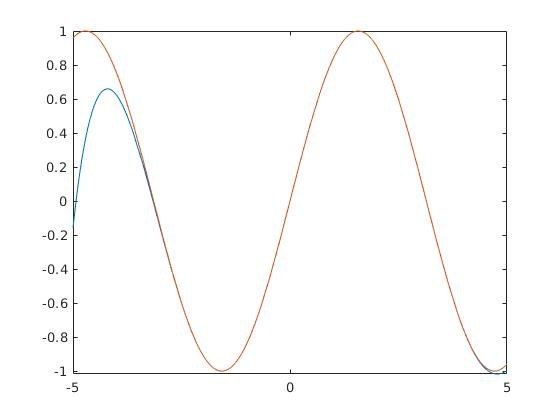
\includegraphics[width=3in]{SinVsS}
        \end{center}
    \end{solution}
\end{questions}
\end{document}
